\documentclass[12pt,a4paper]{report}
\usepackage[utf8]{inputenc}
\usepackage[T1]{fontenc}
\usepackage[french]{babel}
\usepackage{geometry}
\usepackage{pdfpages}
\usepackage{tikz}
\usepackage{array}
\usepackage{longtable}
\usepackage{enumitem}
\usepackage{hyperref}

\geometry{left=2.5cm,right=2.5cm,top=2.5cm,bottom=2.5cm}
\setlist[itemize]{label=--}

\begin{document}

% Le rapport initial est garde comme base pour ne pas changer beaucoup le document.
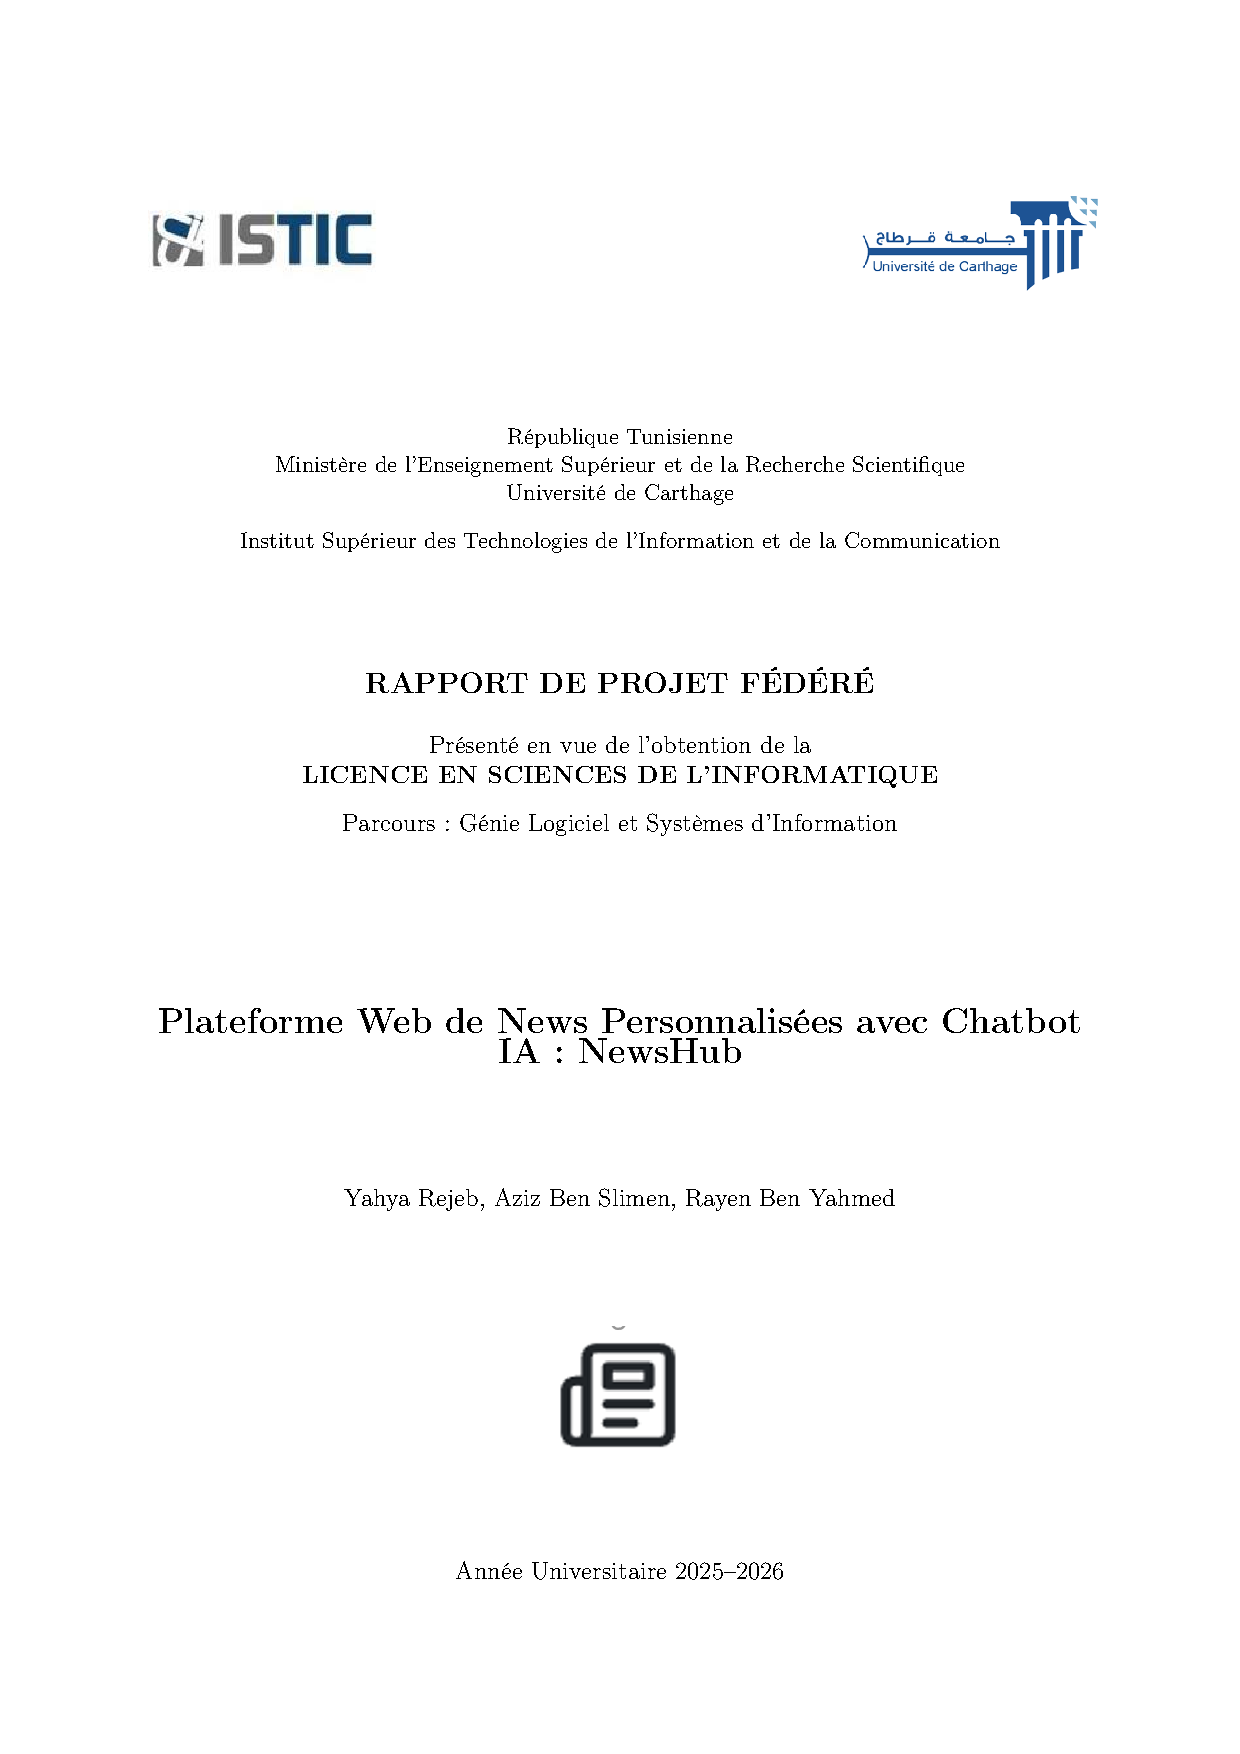
\includepdf[pages=-]{news_v1_original.pdf}

\chapter*{Réalisation du Sprint 1}
\addcontentsline{toc}{chapter}{Réalisation du Sprint 1}
La réalisation du Sprint 1 complète les fonctionnalités principales de la plateforme NewsHub. Cette partie ajoute les interfaces et les traitements liés à l'espace utilisateur, aux favoris, aux commentaires, à l'abonnement premium et au chatbot IA.

\section*{Interfaces réalisées}
\begin{itemize}
\item Interface de gestion du profil : consultation et modification des informations personnelles.
\item Interface des favoris : affichage des actualités enregistrées par l'utilisateur.
\item Interface des commentaires : ajout et consultation des commentaires liés à une actualité.
\item Interface d'abonnement : simulation d'une offre premium.
\item Interface du chatbot : discussion avec l'assistant IA à partir d'une actualité.
\end{itemize}

\section*{Diagramme de déploiement}
\begin{center}
\begin{tikzpicture}[node distance=1.8cm, every node/.style={draw, rounded corners, align=center, minimum width=3cm, minimum height=1cm}]
\node (client) {Navigateur\\Angular};
\node[right of=client, xshift=3cm] (api) {Serveur API\\FastAPI};
\node[right of=api, xshift=3cm] (db) {Base de données\\MySQL};
\node[below of=api] (ollama) {Service IA\\Ollama};
\node[above of=api] (news) {API externe\\Newsdata.io};
\draw[->] (client) -- (api);
\draw[->] (api) -- (db);
\draw[->] (api) -- (news);
\draw[->] (api) -- (ollama);
\end{tikzpicture}
\end{center}

\chapter*{Conclusion générale}
\addcontentsline{toc}{chapter}{Conclusion générale}
Dans ce projet fédéré, nous avons conçu et réalisé NewsHub, une plateforme web d'actualités personnalisées avec chatbot IA. Le système permet à l'utilisateur de consulter des actualités, filtrer le contenu, créer un compte, se connecter, gérer son profil, enregistrer des articles, commenter, s'abonner et discuter avec un assistant intelligent.

La méthode SCRUM nous a permis d'organiser le travail en sprints. Le Sprint 0 a assuré les fonctionnalités de base, telles que l'inscription, la connexion, la consultation et le filtrage des actualités. Le Sprint 1 a enrichi la plateforme avec les fonctionnalités liées au profil, aux favoris, aux commentaires, à l'abonnement et au chatbot.

Sur le plan technique, le projet repose sur une architecture web moderne composée d'un frontend Angular, d'un backend FastAPI, d'une base de données MySQL, d'une API externe d'actualités et d'un service IA local basé sur Ollama.

\section*{Perspectives}
Comme perspectives, nous pouvons proposer l'intégration d'un paiement réel, l'amélioration du système de recommandation, l'ajout de notifications, la mise en place de tests automatisés et le renforcement de la modération des commentaires et des espaces live.

\end{document}
